\chapter{Cost Estimation}
In this section we include a cost estimation for CookingTime application development.
In order to exploit the estimation, we decided to use COCOMO (Constructive Cost Model) model.
The usage of this analysis tool allows us to determine the time required for the development of this type of application.
First of all, we have to decide what type of project we are producing in order to take the right estimation parameters, according to the following table.\\
\begin{table}[H]
	\centering
	\begin{tabular}{|l|c|c|c|c|}
	\hline
	\textbf{Software Project}& \textbf{a}& \textbf{b}& \textbf{c}& \textbf{d}\\
	\hline
	Organic & 2.40 & 1.05 & 2.50 & 0.38 \\
	\hline
	Semi-detached & 3.00 & 1.12 & 2.50 & 0.35 \\
	\hline
	Embedded & 3.60 & 1.20 & 2.50 & 0.32 \\
	\hline
	\end{tabular}
	\caption{COCOMO coefficients}
\end{table}
The classes of COCOMO represent different difficulties of the product and experiences of developers, especially:
\begin{itemize}
	\item \textbf{Organic} It means small project done by small teams with a good experience and low constraints.
	\item \textbf{Semi-Detached} It means project with a significant large team with different experiences and medium constraints.
	\item \textbf{Embedded} It means we have tight constraints and a mixture of Organic and Semi-Detached classes of projects.
\end{itemize}
Then we can consider the equation to represent the effort spent:\\
\begin{center}
$ effort = a * KLOC ^{b}$\\
$ duration = c * effort^{d}$\\
\end{center}
where \textbf{KLOC} are the estimated number of thousand lines of code, \textbf{effort} expressed in man-months and the duration is the time estimated to be taken in order to develop the application.\\
Even if it was the first time we developed a mobile application and the first time we used the Dart programming language, we already had good bases in coding.
Moreover, the project is simple and without tight constraints, so we can consider our project as organic, also because we have a team composed by only two students.\\
We can start retrieving from our Github repository the number of Kilo Line Of Code (KLOC) as shown in the following figure.\\
\begin{figure}[H]
		\begin{center}
			\centering
			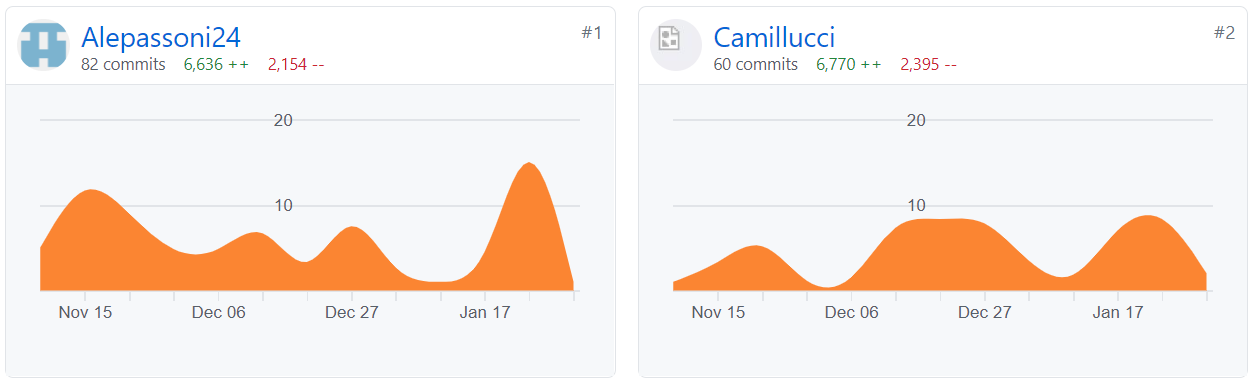
\includegraphics[width=0.8\textwidth]{img/RepoInsights.png}
			\caption{GitHub Contributions}
		\end{center}
	\end{figure}
Then according to Organic project coefficient we can evaluate the effort applied and the predicted development time:

\begin{itemize}
	\item \textbf{KLOC} = 10
	\item \textbf{a} = 2.40
	\item \textbf{b} = 1.05
	\item \textbf{c} = 2.50
	\item \textbf{d} = 0.38
\end{itemize}

\begin{center}
$ effort = a * (KLOC)^{b} = 2.40 * 9^{1.05} = 24.1 $\\
$ duration = c * effort^{d} = 2.50 * 24.1 ^{0.38} = 8.3 $\\
\end{center}

The estimated development time by COCOMO is about 8 months.
Considering the time we spent and the size of the team, it is approximately right and coherent with our effort.
